\documentclass[book,openany]{jlreq}

%---------- package ----------% 
\usepackage{graphicx}
\usepackage[pdfencoding=auto]{hyperref}
\usepackage{booktabs}
%\usepackage{subfig}
\usepackage{pifont}
\usepackage{url}
\usepackage{cite}
\usepackage{ulem}
\usepackage{siunitx}
\usepackage{float}
\usepackage{tcolorbox}
\tcbuselibrary{breakable}
\usepackage{cancel}
\usepackage{color}

%--- physics2 ---%
\usepackage{physics2}
\usephysicsmodule{ab}   % 括弧サイズの自動調整
\usephysicsmodule{ab.braket}    % braket記法
\usephysicsmodule{diagmat}  % 対角行列
\usephysicsmodule[showleft=2,showtop=2]{xmat}   % n×m行列
%--- physics2 END ---%
% 数式環境
\usepackage{amsmath,amssymb,amsthm}
% ベクトル
\usepackage{bm}
%--- 微分演算子 ---%
\usepackage{fixdif}
\usepackage{derivative}
%--- 微分演算子 END ---%
% 花文字
\usepackage{mathrsfs}
%
%---------- package END ----------% 

%---------- newcommand ----------% 
% 積分値の評価
\newcommand{\eval}[1]{\left.#1\right|}
% Landau記号
\newcommand{\order}[1]{\mathcal{O}\ab(#1)}
%--- physicsパッケージの\vbコマンドを再現 --%
\makeatletter
\newcommand\vb{\@ifstar\boldsymbol\mathbf}
\newcommand\va[1]{\@ifstar{\vec{#1}}{\vec{\mathrm{#1}}}}
\newcommand\vu[1]{%
\@ifstar{\hat{\boldsymbol{#1}}}{\hat{\mathbf{#1}}}}
\makeatother
%--- physicsパッケージの\vbコマンドを再現 END --%
%--- 勾配・発散・回転 ---%
% 勾配
\DeclareMathOperator{\grad}{\nabla}
% 発散
% \divが「÷」と競合するため再定義
\DeclareMathOperator{\divergence}{\nabla\cdot}
\let\divisionsymbol\div 
\renewcommand{\div}{\divergence} 
% 回転
\DeclareMathOperator{\rot}{\nabla\times}
%--- 勾配・発散・回転 END ---%
% 実部
\renewcommand{\Re}{\operatorname{Re}}
% 虚部
\renewcommand{\Im}{\operatorname{Im}}
% トレース
\newcommand{\Tr}{\operatorname{Tr}}
% rank
\newcommand{\rank}{\operatorname{rank}}
% \mqtyコマンド
\newcommand{\mqty}[1]{\begin{matrix}#1\end{matrix}}
%
\renewcommand{\CancelColor}{\color{red}}
%
%---------- newcommand END ----------% 

% \usepackage[hang,small,bf]{caption}
% \usepackage[subrefformat=parens]{subcaption}
% \captionsetup{compatibility=false}

\theoremstyle{definition}
\newtheorem{theorem}{定理}[chapter]
\newtheorem*{theorem*}{定理}
\newtheorem{definition}[theorem]{定義}
\newtheorem*{definition*}{定義}

\usepackage{xcolor}
\hypersetup{
  bookmarksnumbered=true,
  colorlinks=true,
  citecolor=red,
  linkcolor=blue,
  urlcolor=orange,
}

\begin{document}
\title{Crowbar回路}
\author{吉本 伸一}
\maketitle
\tableofcontents

\chapter{SuperKEKBのクライストロン電源}
\section{SuperKEKBのRFシステムの概要}

%
\begin{figure}[htbp]
  %\begin{figure}[!htt]
  \begin{center}
    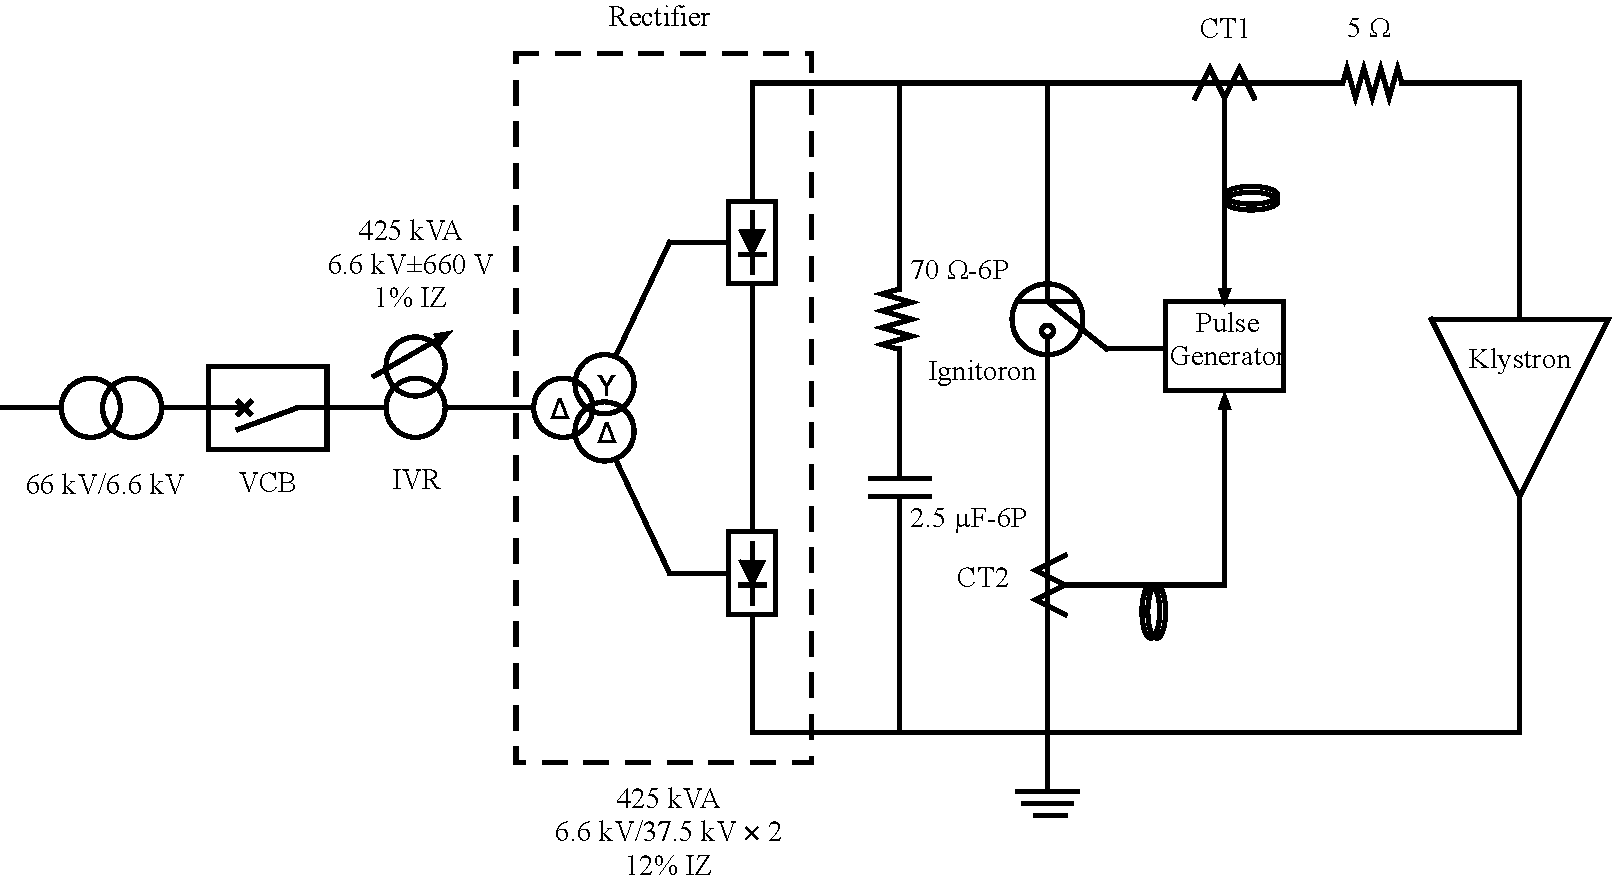
\includegraphics[width=12cm]{figs/Crowbar_Circuit.pdf}
    \caption{クローバー回路.}
    \label{fig:CrowbarCircuit}
  \end{center}
\end{figure}

\chapter{クローバー短絡試験}

\begin{figure}[htbp]
  %\begin{figure}[!htt]
  \begin{center}
    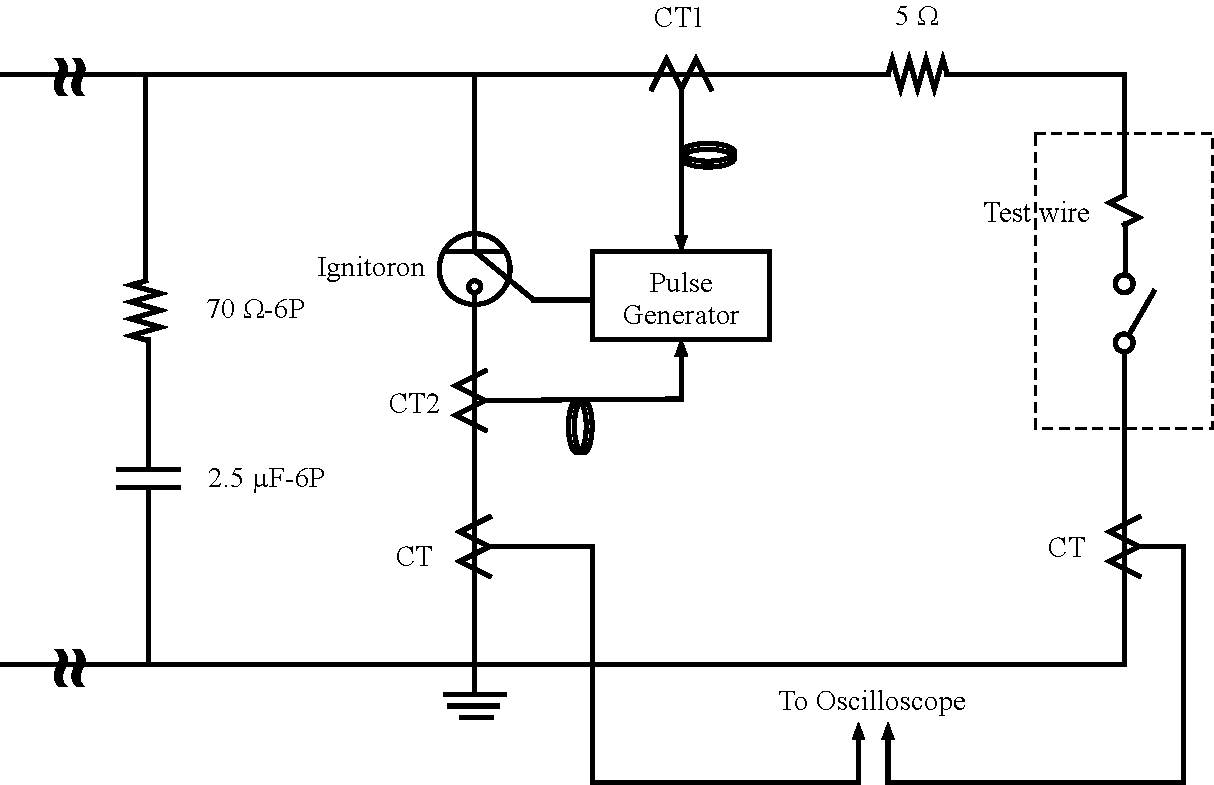
\includegraphics[width=12cm]{figs/Crowbar_Test.pdf}
    \caption{短絡試験時のセットアップ.}
    \label{fig:CrowbarTest}
  \end{center}
\end{figure}
%
クローバー回路の健全性を確認するため、毎年夏のメンテナンス時に短絡試験を行なっている。(図\ref{fig:CrowbarTest})が短絡試験を行う時のセットアップである。短絡電流とクローバー電流を測定する為にCT(PEARSON\texttrademark\, CURRENT MONITOR MODEL 3025)を使用している。テストワイヤー($0.35\,\phi,\, 200\,\mathrm{mm}$の銅線)と短絡のためのギャップは安全の為、短絡試験器の中に収めてる。(図\ref{fig:Tanraku})
%
\begin{figure}[htbp]
  \centering
  \begin{minipage}[b]{0.45\linewidth}
    \centering
    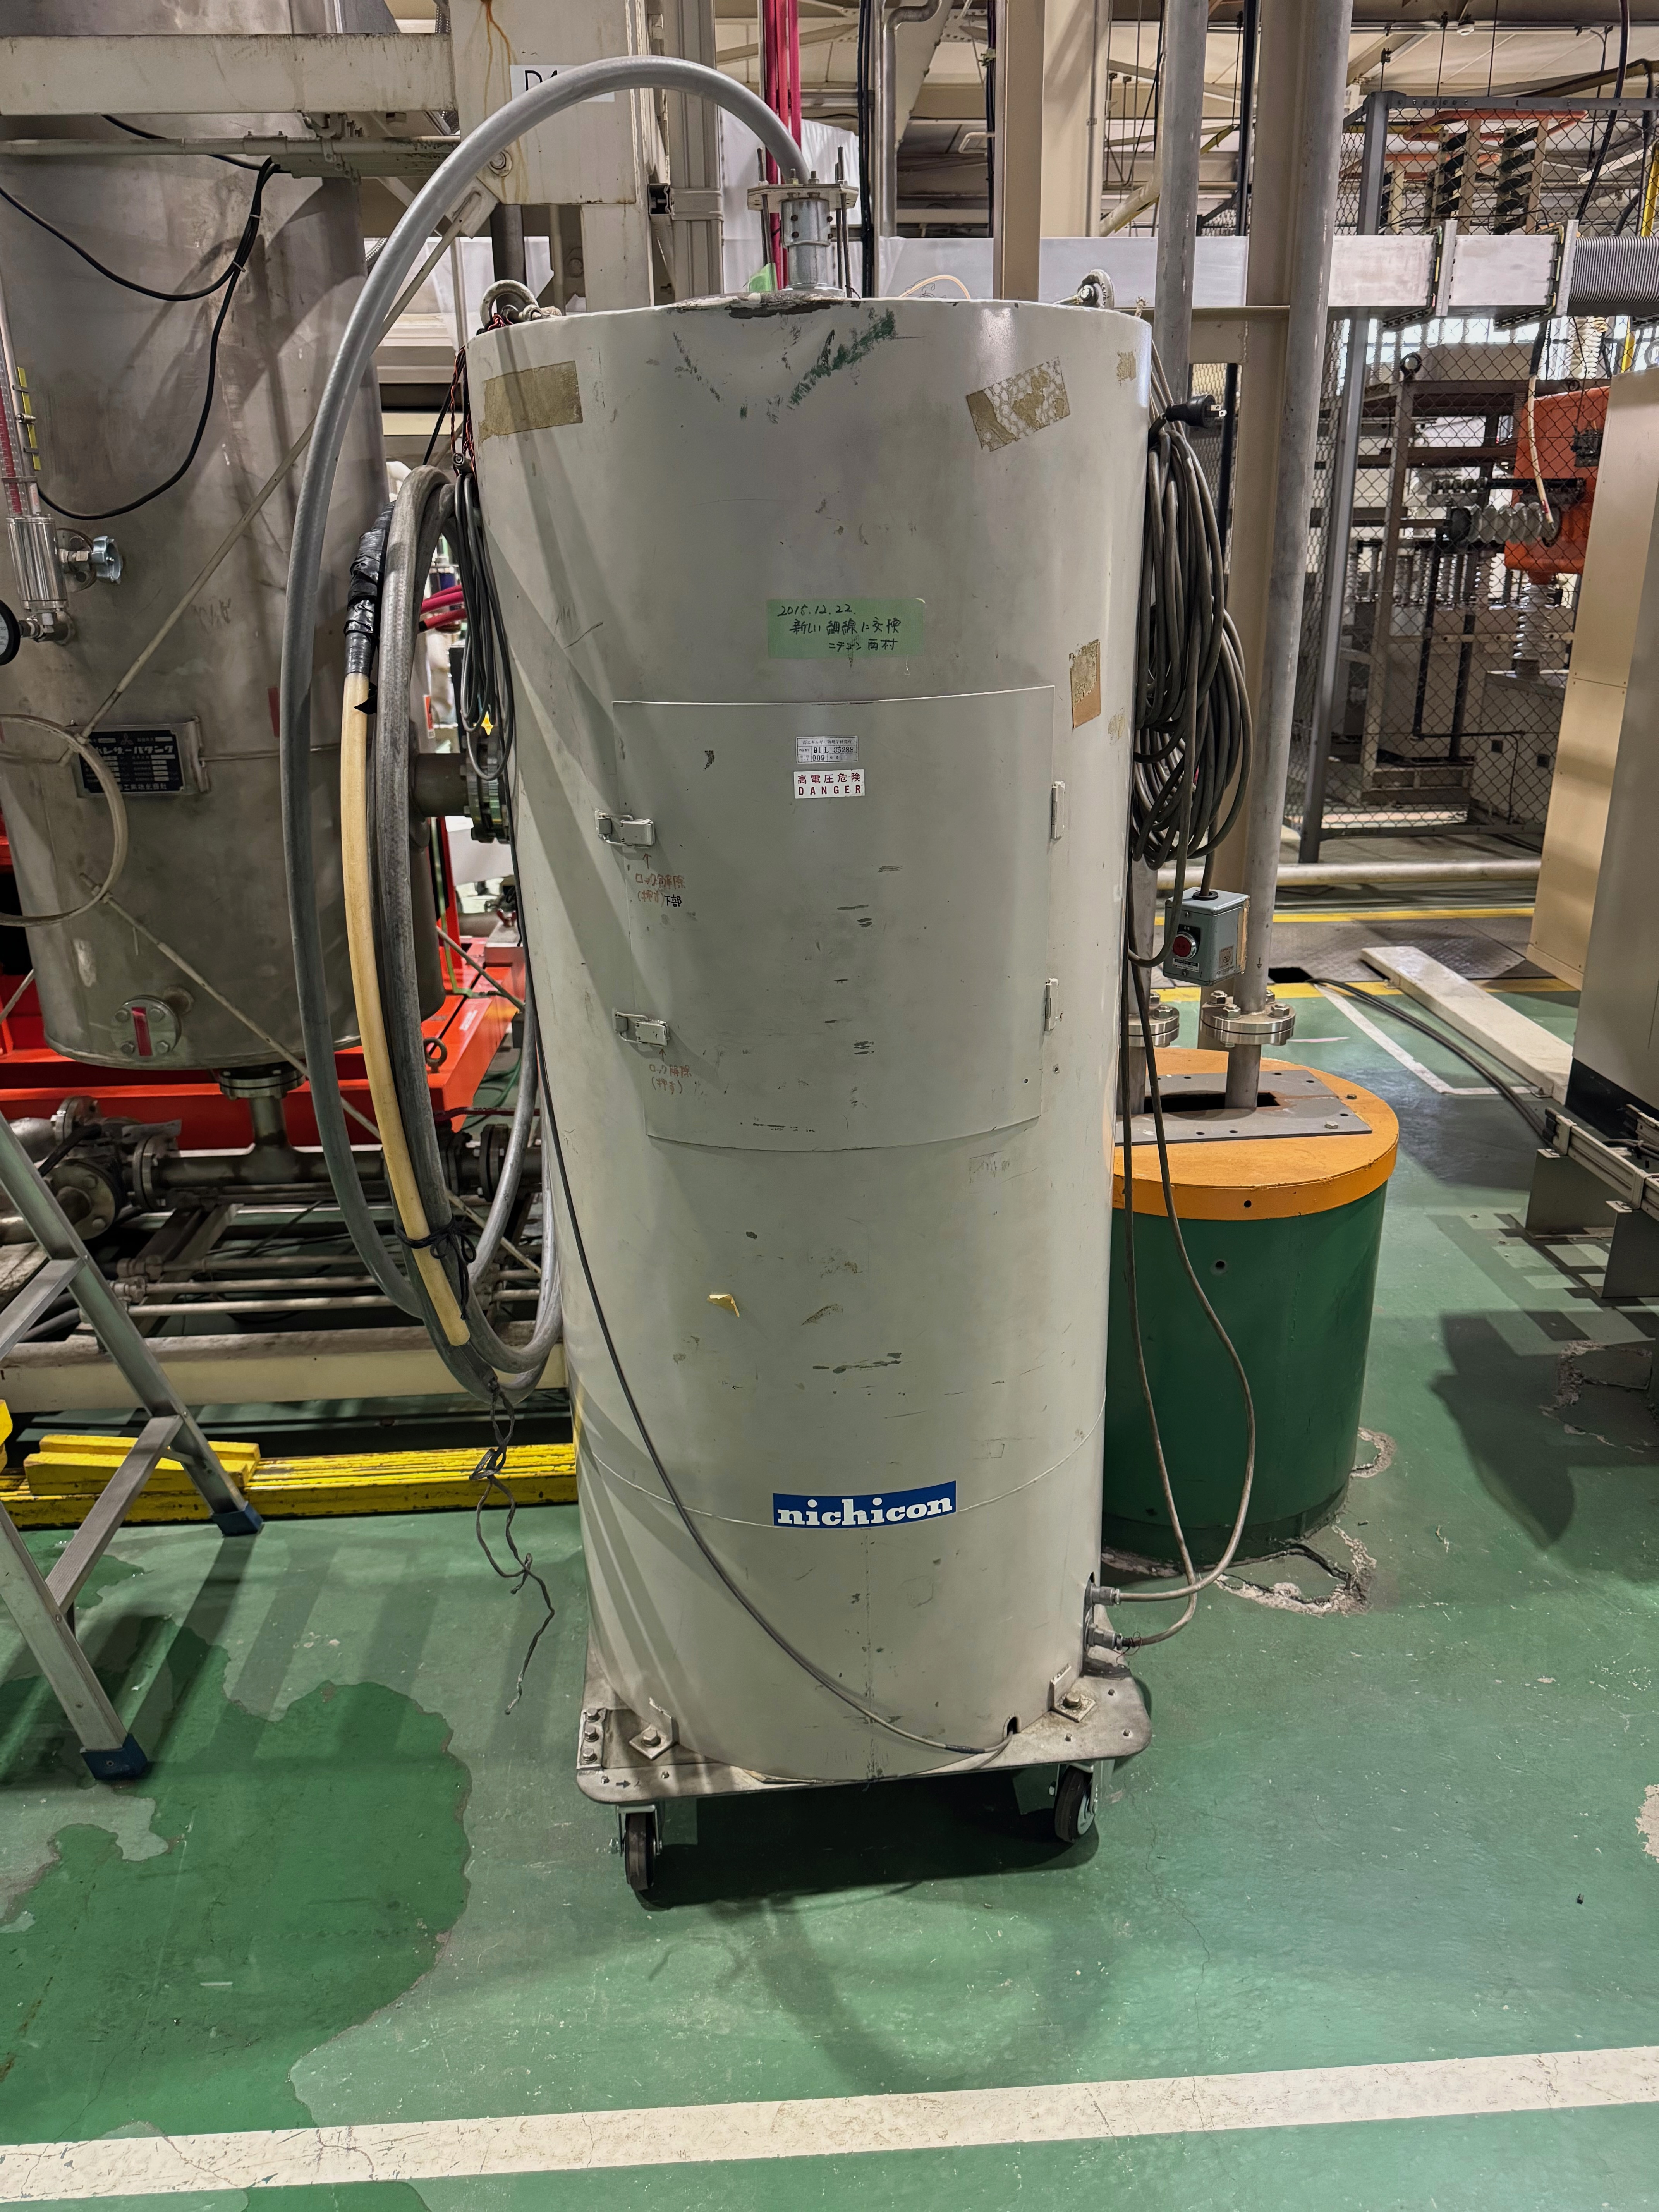
\includegraphics[width=0.9\columnwidth]{./figs/Tanraku1.jpeg}
  \end{minipage}
  \begin{minipage}[b]{0.45\linewidth}
    \centering
    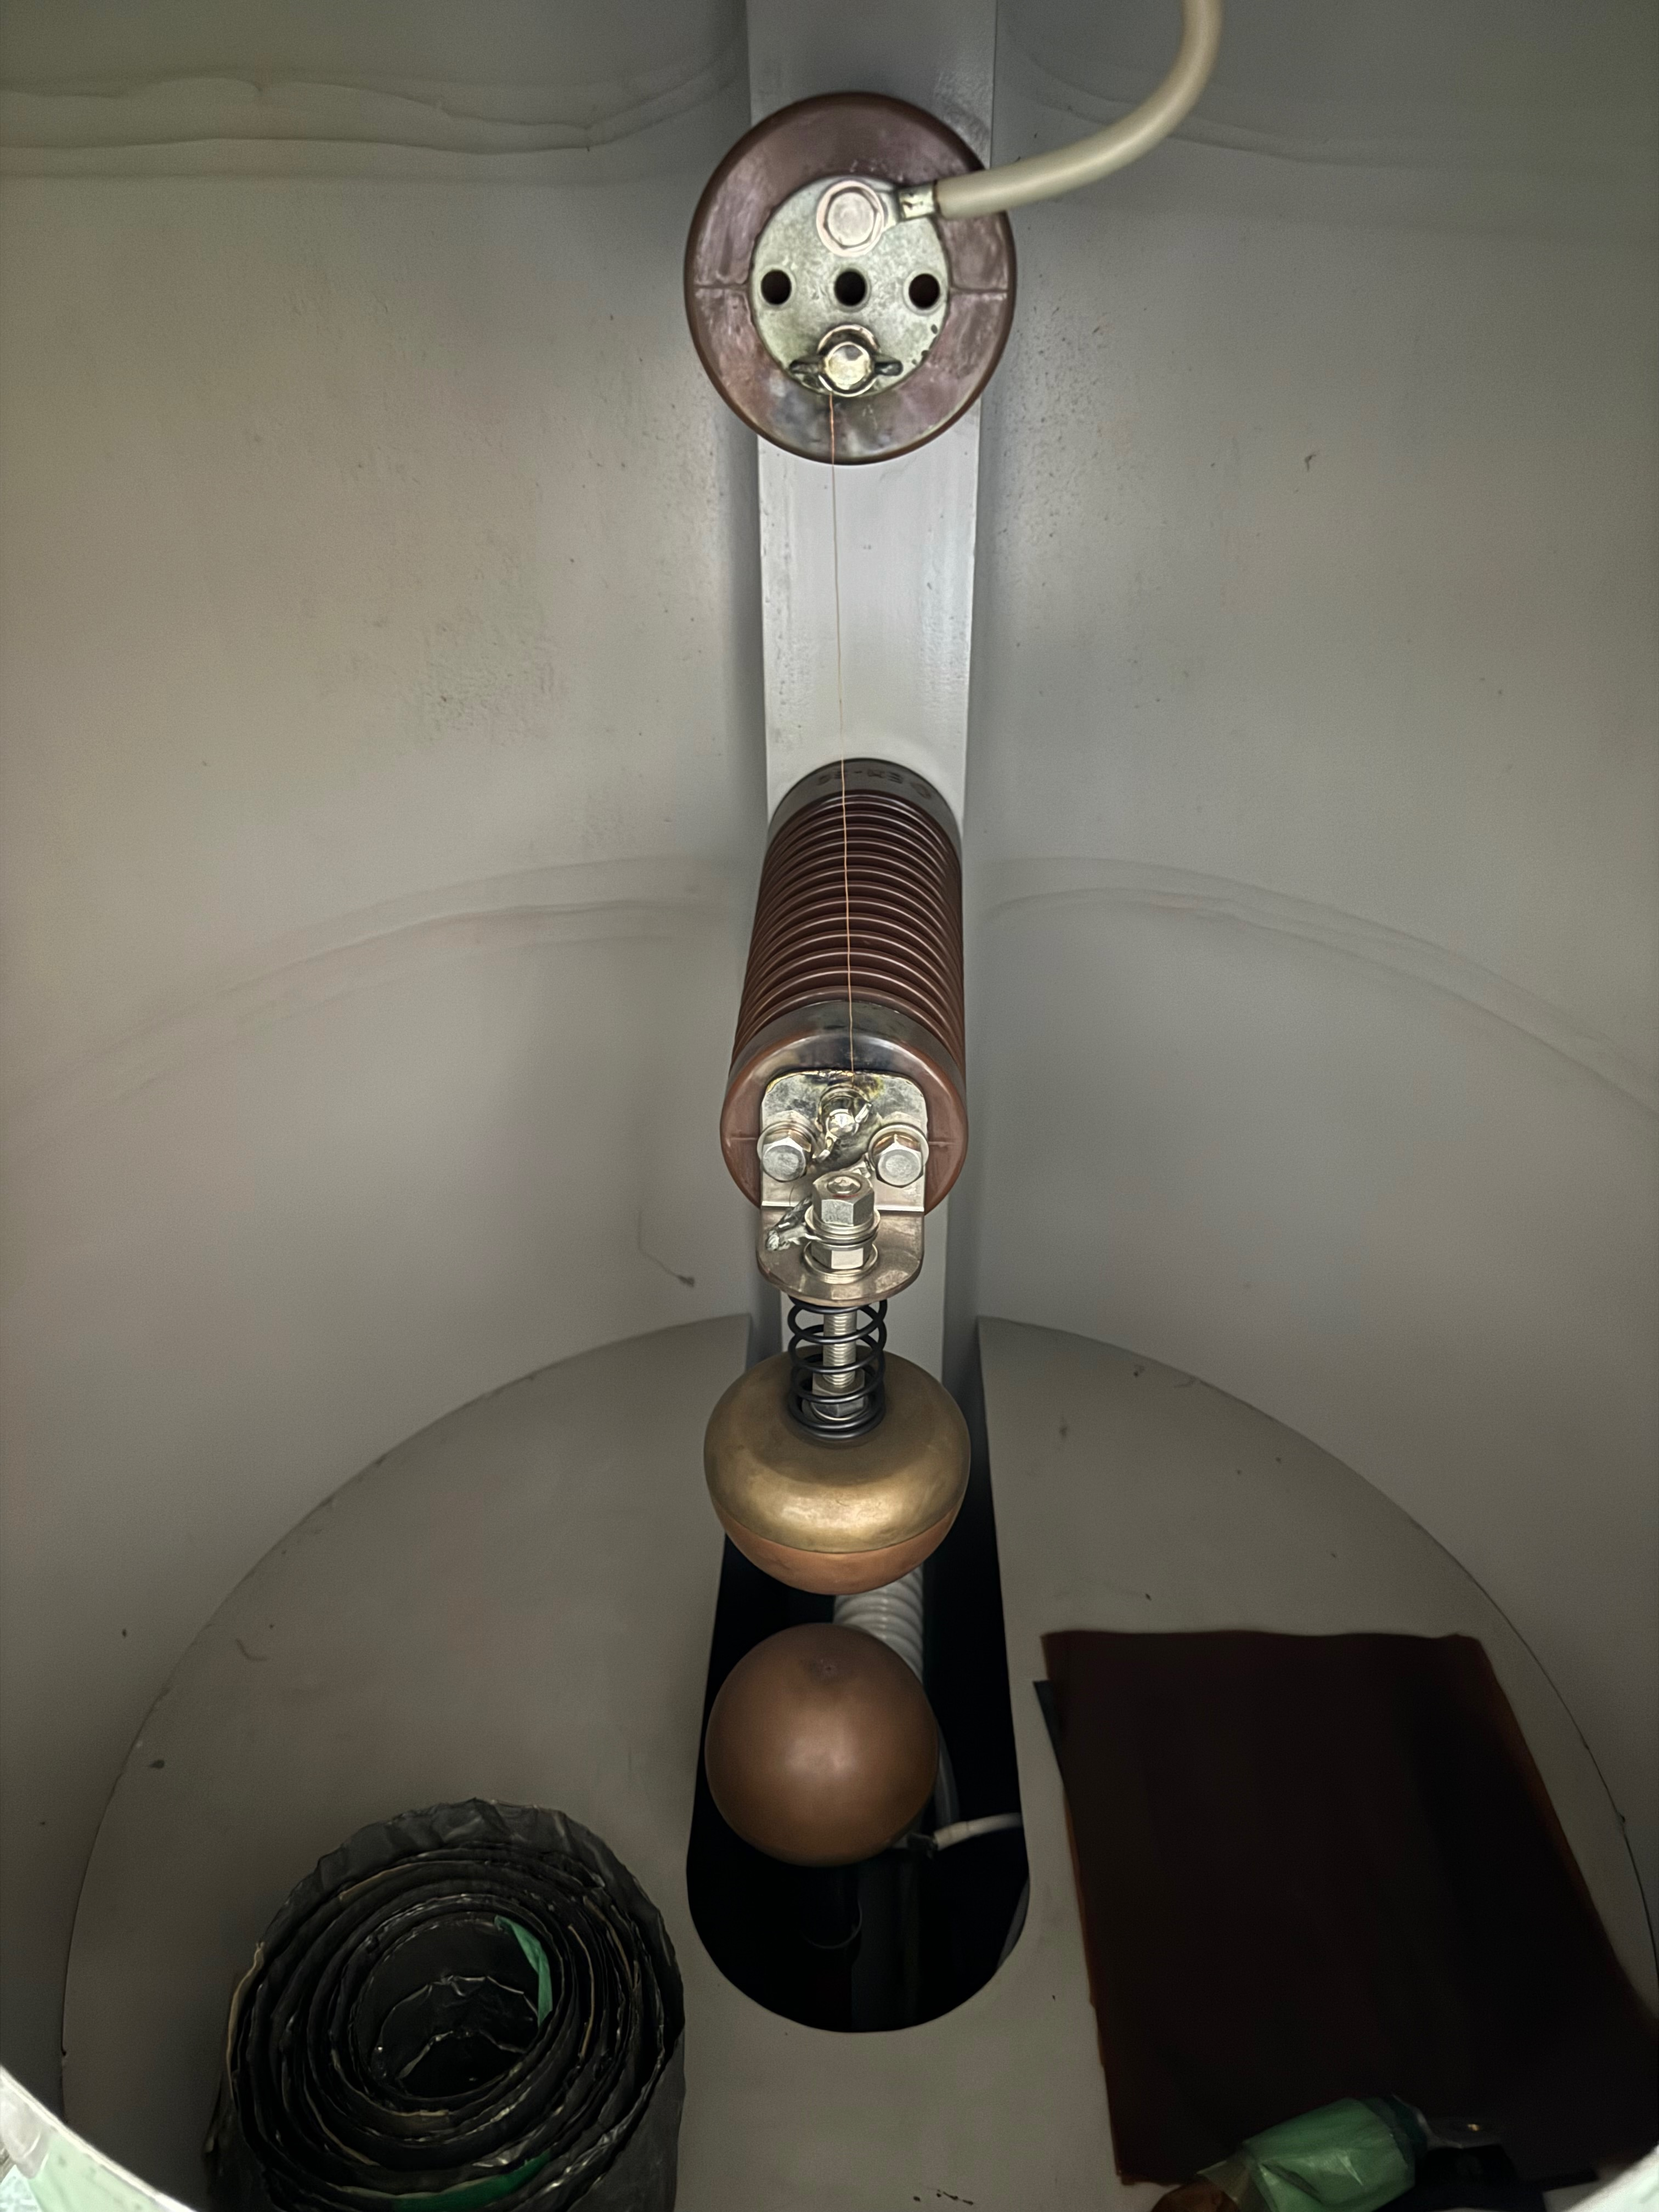
\includegraphics[width=0.9\columnwidth]{./figs/Tanraku2.jpeg}
  \end{minipage}
  \caption{短絡試験器 (左 : 全体, 右 : 短絡試験機内部の銅細線と短絡用ギャップ)}
  \label{fig:Tanraku}
\end{figure}

\section{オシロの測定系について}
短絡電流とクローバー電流の測定に使用しているピアソンのCTの出力は\SI{0.025}{V\per A}、つまり\SI{40}{A\per V}となる。このままでは電圧が大きすぎるので、\SI{10}{\decibel}のアッテネーターを入れて$1/10$にしている。また、CTの出力インピーダンスを$R_o$とし、オシロの入力インピーダンスを$R_i$とすると、オシロで測定する電圧$V_m$はCTから送られる電圧$V$とするとき
%
\begin{equation}
  V_m = \frac{R_i}{(R_i + R_o)} V
\end{equation}
%
となる。今オシロ側はインピーダンスマッチングするため\SI{50}{\ohm}のスルータイプのターミネーターで終端してるから$R_o=R_i=\SI{50}{\ohm}$となって$V_m=V/2$となり、CTで測定された電圧$V$はオシロで測定された電圧$V_m$の2倍になる事に注意。したがって、測定結果は\SI{800}{A\per V}となる。
%
\begin{figure}[htbp]
  \begin{center}
    \includegraphics[width=12cm]{figs/Term_Att.pdf}
    \caption{ターミネーターとアッテネーター.}
    \label{fig:Term_Att}
  \end{center}
\end{figure}

\section{短絡試験の等価回路}
\begin{figure}[htbp]
  %\begin{figure}[!htt]
  \begin{center}
    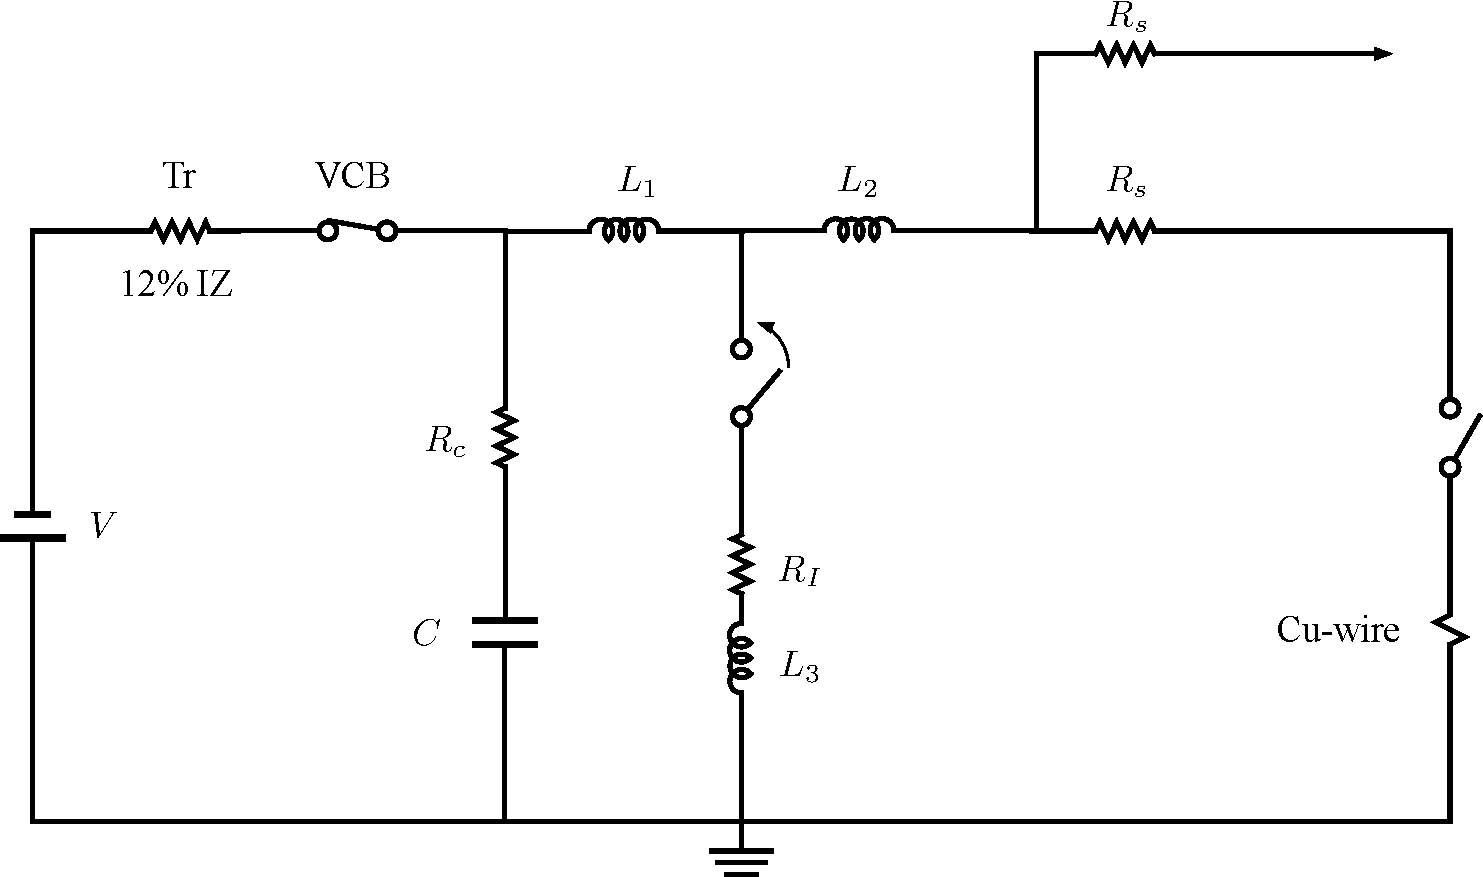
\includegraphics[width=12cm]{figs/Equivalent_Circuit.pdf}
    \caption{短絡試験時の等価回路.}
    \label{fig:Equivalent_Circuit}
  \end{center}
\end{figure}

\section{電源からの注入エネルギー}
%
まずは、クローバー動作時に電源から注入されるエネルギーを考える。

\begin{figure}[htbp]
  %\begin{figure}[!htt]
  \begin{center}
    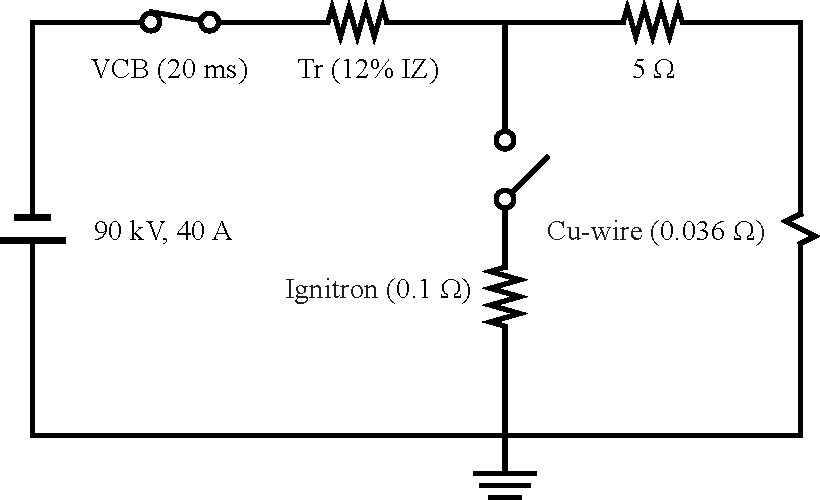
\includegraphics[width=12cm]{figs/FromPS.pdf}
    \caption{短絡試験時の等価回路.}
    \label{fig:FromPS}
  \end{center}
\end{figure}

\clearpage

\section{クローバー動作前}

クローバー動作前の等価回路は(図\ref{fig:BeforeCrowbar})のようになる。

\begin{figure}[htbp]
  %\begin{figure}[!htt]
  \begin{center}
    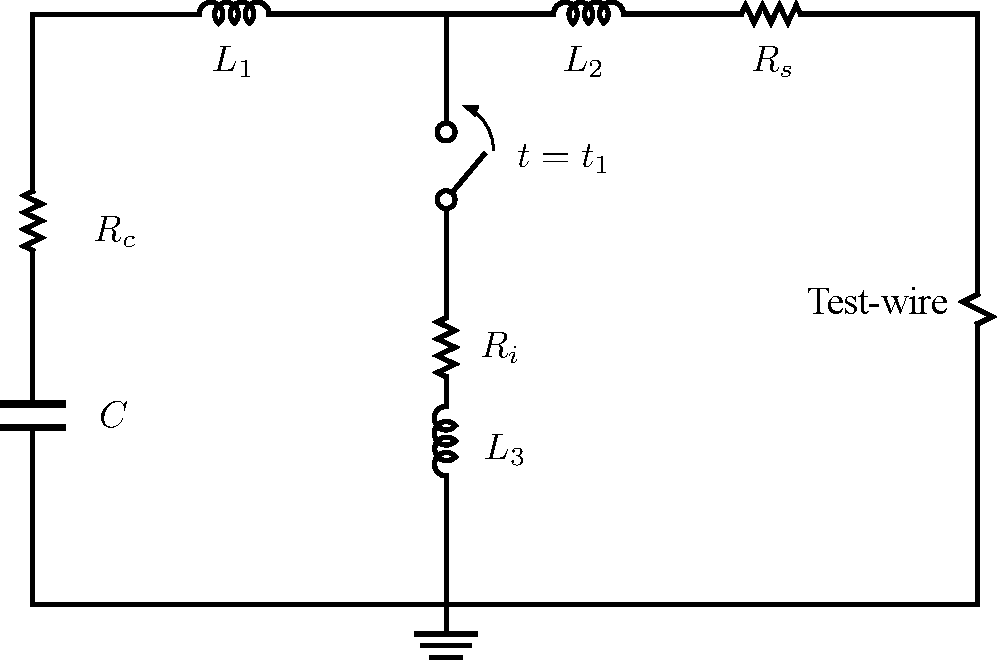
\includegraphics[width=12cm]{figs/BeforeCRB.pdf}
    \caption{クローバー動作前の等価回路.}
    \label{fig:BeforeCrowbar}
  \end{center}
\end{figure}
%
この回路の微分方程式は
%
\begin{equation}
  (L_1+L_2) \frac{di(t)}{dt} + (R_c+R_s) i(t) + \frac{1}{C} \int i(t) dt = 0
\end{equation}
%
両辺を時間$t$で微分すると
%
\begin{equation}
  (L_1+L_2)\frac{d^2i(t)}{dt^2} + (R_c+R_s) \frac{di(t)}{dt} + \frac{1}{C} i(t) = 0
  \label{eq:differential_eq}
\end{equation}
%
特性方程式
%
\begin{equation}
  (L_1+L_2)\lambda^2 + (R_c+R_s)  \lambda + \frac{1}{C} = 0
  \label{eq:chara_eq}
\end{equation}
%
の判別式$D$は
%
\begin{equation}
  D = (R_c+R_s)^2 -\frac{4 (L_1+L_2)}{C}
\end{equation}
%
ここで、$L$は十分小さいので、$D>0$となり(\ref{eq:chara_eq})は異なる2つの実数解をもつ。その解を$\lambda_1$と$\lambda_2$とすると、微分方程式(\ref{eq:differential_eq})の一般解は$A$と$B$を定数として次のように書ける。
%
\begin{equation}
  i(t) = A e^{\lambda_1 t} + B e^{\lambda_2 t}
\end{equation}
%
初期条件 $t=0$で$i(0)=0$より
%
\begin{equation}
  i(0) = A + B = 0
\end{equation}
%
$t=0$でコンデンサの電圧が$V_0$とすると
%
\begin{equation}
  (L_1+L_2)\left. \frac{di(t)}{dt} \right|_{t=0}= V_0
\end{equation}
%
これより、
%
\begin{equation}
  A = -B = \frac{V_0}{(\lambda_1 - \lambda_2)(L_1+L_2)}
\end{equation}
%
したがって、回路に流れる電流は次のようになる。
%
\begin{equation}
  i(t) = \frac{V_0}{(\lambda_1 - \lambda_2)(L_1+L_2)} \left(e^{\lambda_1 t} - e^{\lambda_2 t}\right)
\end{equation}

\section{クローバー動作以降}

クローバー動作以降の等価回路は(図\ref{fig:AfterCrowbar})のようになる。
%
\begin{figure}[htbp]
  %\begin{figure}[!htt]
  \begin{center}
    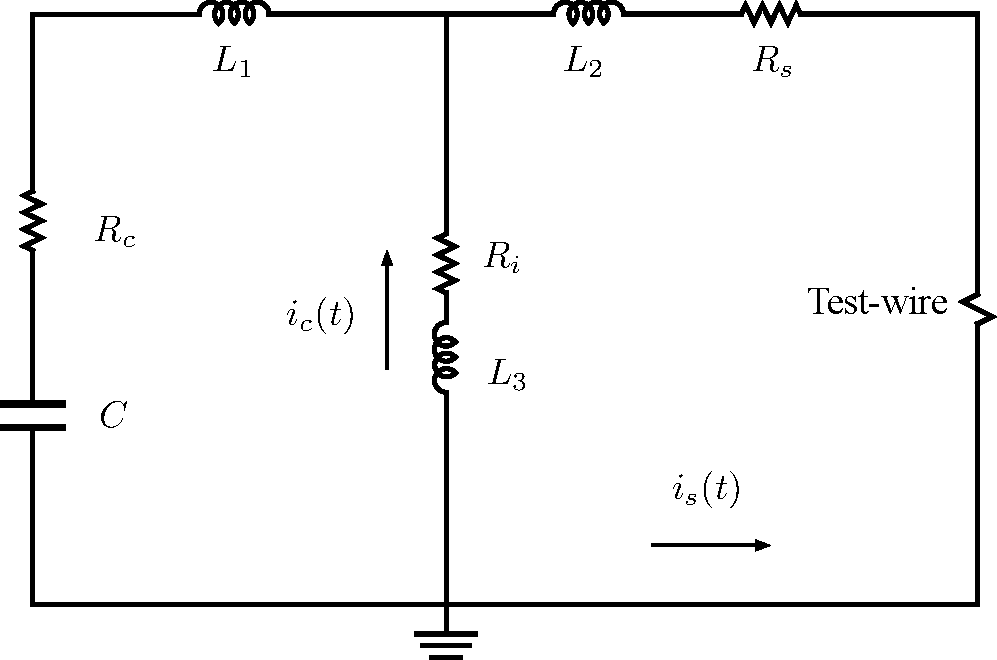
\includegraphics[width=12cm]{figs/AfterCRB.pdf}
    \caption{クローバー動作後の等価回路.}
    \label{fig:AfterCrowbar}
  \end{center}
\end{figure}
%
この回路の左側のループを考えると、クローバー電流$i_c(t)$微分方程式は
%
\begin{equation}
  (L_1+L_3) \frac{di_c(t)}{dt} + (R_c+R_i) i_c(t) + \frac{1}{C} \int i(t)_c dt = 0
\end{equation}
%
両辺を時間$t$で微分すると
%
\begin{equation}
  (L_1+L_3)\frac{d^2i_c(t)}{dt^2} + (R_c+R_i) \frac{di_c(t)}{dt} + \frac{1}{C} i_c(t) = 0
  \label{eq:differential_eq2}
\end{equation}
%
特性方程式
%
\begin{equation}
  (L_1+L_3)\lambda^2 + (R_c+R_i)  \lambda + \frac{1}{C} = 0
  \label{eq:chara_eq2}
\end{equation}
%
の判別式$D$は
%
\begin{equation}
  D = (R_c+R_i)^2 -\frac{4 (L_1+L_3)}{C}
\end{equation}
%
ここで、$L$は十分小さいので、$D>0$となり(\ref{eq:chara_eq2})は異なる2つの実数解をもつ。その解を$\lambda_1$と$\lambda_2$とすると、微分方程式(\ref{eq:differential_eq2})の一般解は$A$と$B$を定数として次のように書ける。
%
\begin{equation}
  i_c(t) = A e^{\lambda_1 t} + B e^{\lambda_2 t}
\end{equation}
%
初期条件 $t=t_1$で$i_c(t_1)=0$より
%
\begin{equation}
  i_c(t_1) = A e^{\lambda_1 T_1} + B e^{\lambda_2 t_2} = 0
\end{equation}
%
$t=t1$でコンデンサの電圧が$V_1$とすると
%
\begin{equation}
  (L_1+L_3)\left. \frac{di_c(t)}{dt} \right|_{t=t_1}= V_1
\end{equation}
%
したがって、
\begin{equation}
  A = -B = \frac{V_1}{(\lambda_1 - \lambda_2)(L_1+L_3)}
\end{equation}
%
%
これより、クローバー電流 $i_c(t)$は次のようになる。
\begin{equation}
  i_c(t) = \frac{V_1}{(\lambda_1-\lambda_2)L}\bigl\{e^{\lambda_1(t+t_1)}-e^{\lambda_2(t+t_1)}\bigr\}
\end{equation}

次に右側のループを考えると、

\begin{equation}
  L \frac{di(t)}{dt} + R i(t) = 0
\end{equation}
%
この方程式を、初期条件$t=t_1$で$i(t_1)=I_0$の元に解くと
%
\begin{equation}
  i(t) = I_0 e^{-(t-t_1)/\tau}\;,\quad \tau = \frac{L}{R}
\end{equation}
%
となる。

また、クローバー電流も$L$, $C$, $R$の直列回路を考えればよく、初期条件としては$t=t_1$で$i(0)=0$、コンデンサの電圧$V_0$となるので同様に解析でき、
%
\begin{equation}
  A e^{\lambda_1 t_1}+B e^{\lambda_2 t_1} = 0\;,\qquad L\left .\frac{di(t)}{dt} \right|_{t=t_1}=V_0
\end{equation}
%
これより、クローバー電流 $i_c(t)$は次のようになる。
\begin{equation}
  i_c(t) = \frac{V_0}{(\lambda_1-\lambda_2)L}\bigl\{e^{\lambda_1(t+t_1)}-e^{\lambda_2(t+t_1)}\bigr\}
\end{equation}
%
\chapter{測定データの解析}

\clearpage

\section{physics2練習帳}

\begin{equation}
  \ab( \frac{1}{2} )\quad
  \ab[ \frac{1}{2} ]\quad
  \ab< \frac{1}{2} >\quad
  \ab| \frac{1}{2} |\quad
  \ab\| \frac{1}{2} \|\quad
  \ab\{ \frac{1}{2} \}\quad
  \sin \ab( \frac{\pi}{2} )
\end{equation}

微分記号
%
\begin{equation}
  \d x\quad
  \odv{}{x}\quad
  \odv{f}{x}\quad
  \odv[order=n]{f}{x}\quad
  \odv{f}/{x}\quad
  \odv*{f(x)}{x}
\end{equation}

偏微分
%
\begin{equation}
  \pdv{}{x}\quad
  \pdv{f}{x}\quad
  \pdv{f}{x, y}\quad
  \pdv[order=n]{f}{x}\quad
  \pdv{f}/{x}\quad
  \pdv*{f(x,y,z)}{x}\quad
  \pdv[order={2, 1, 2}]{f}{x, y, z}\quad
\end{equation}

Vector
%
\begin{equation}
  \vb{v}\quad
  \va{v}\quad
  \vu{v}\quad
  \grad \phi\quad
  \div \bm{x}\quad
  \rot \bm{x}\quad
  a \divisionsymbol b\quad
\end{equation}

operator
%
\begin{equation}
  \Re \ab[ f(z) ]\quad
  \Im \ab[ f(z) ]\quad
  \Tr \ab[ A ]\quad
  \rank \ab[ A ]\quad
\end{equation}

braket
%
\begin{equation}
  \ket|\psi> \quad
  \bra<\phi|\quad
  \braket<\phi|\psi>\quad
  \ketbra|\psi><\phi|\quad
  \braket<\psi>\quad
  \braket<\psi|A|\psi>\quad
  \ab| { \braket<\psi|A|\psi> } |
\end{equation}

matrix
%
\begin{equation}
  \mqty{ a&b\\c&d }\quad % 括弧無し
  \ab( \mqty{ a&b\\c&d }  )\quad % 小括弧()
  \ab[ \mqty{ a&b\\c&d }  ]\quad % 大括弧[ ]
  \ab| \mqty{ a&b\\c&d }  |\quad % 行列式| |
\end{equation}


\begin{thebibliography}{9}
  \bibitem{Ono}
  M. Ono et al., TRISTAN RF system with normal conducting cavity, KEK Internal 87-6 (1987)
\end{thebibliography}
%
\end{document}